\subsection{STREAMICE Package}
\label{sec:pkg:streamice}
\begin{rawhtml}
<!-- CMIREDIR:package_streamice: -->
\end{rawhtml}

Authors: Daniel Goldberg

%----------------------------------------------------------------------
\subsubsection{Introduction}


Package ``streamice'' provides a dynamic land ice model for MITgcm.

%----------------------------------------------------------------------

\subsubsection{Equations Solved}

As of now, the model tracks only 3 variables: $x$-velocity ($u$), $y$-velocity
($v$), and thickness ($h$). There is also a variable that tracks coverage of
fractional cells, discussed...

By default the model solves the Shallow Shelf approximation (SSA) for velocity.
The SSA is appropriate for floating ice (ice shelf) or ice flowing over a
low-friction bed (e.g. MacAyeal, 1989). The SSA consists of the $x$-momentum
balance:
\begin{equation}
\label{eq:xmom}
 \partial_x(h\nu(4\dot{\varepsilon}_{xx}+2\dot{\varepsilon}_{yy})) +
\partial_y(2h\nu\dot{\varepsilon}_{xy}) - \tau_{bx} = \rho g h s_x 
\end{equation}
the $y$-momentum balance:
\begin{equation}
\label{eq:ymom}
 \partial_x(2h\nu\dot{\varepsilon}_{xy}) +
\partial_y(h\nu(4\dot{\varepsilon}_{yy}+2\dot{\varepsilon}_{xx})) - \tau_{by} =
\rho g h s_y.
\end{equation}
From the velocity field, thickness evolves according to the continuity equation:
\begin{equation}
\label{eq:contEq}
 h_t + \nabla\cdot(h\vec{u}) = -\dot{b},
\end{equation}
Where $\dot{b}$ is a basal mass balance (e.g. melting due to contact with the
ocean), positive where there is melting. Surface mass balance is not considered,
since {\tt pkg/streamice} is intended for localized areas (tens to hundreds of
kilometers) over which the integrated effect of surface mass balance is
generally small. Where ice is grounded, surface elevation is given by 
\begin{equation}
 s = R + h,
\end{equation}
where $R(x,y)$ is the bathymetry, and the basal elevation $b$ is equal to $R$.
If ice is floating, then the assumption of hydrostasy and constant density gives
\begin{equation}
 s = (1-\frac{\rho}{\rho_w} h,
\end{equation}
where $\rho_w$ is a representative ocean density, and $b=-(\rho/\rho_w)h$. Again
by hydrostasy, floation is assumed wherever
\begin{equation}
 h \leq -\frac{\rho_w}{\rho}R
\end{equation}
is satisfied. Floatation criteria is stored in \texttt{float\_frac\_streamice}, equal to 1 where ice is at floatation.

The strain rates $\varepsilon_{ij}$ are generalized to the case of orthogonal
curvilinear coordinates, to include the "metric" terms that arise when casting
the equations of motion on a sphere or projection on to a sphere (see {\tt
pkg/SEAICE}, 6.6.2.4.8 of the MITgcm documentation). Thus
\begin{align}
 \dot{\varepsilon}_{xx} = & u_x + k_1 v, \notag \\
 \dot{\varepsilon}_{yy} = & v_y + k_1 u, \notag \\ 
 \dot{\varepsilon}_{xy} = & \frac{1}{2}(u_y+v_x) + k_1 u + k_2 v. \notag 
\end{align}
$\nu$ has the form arising from Glen's law
\begin{equation}
 \nu =
\frac{1}{2}A^{-\frac{1}{n}}\left(\dot{\varepsilon}_{xx}^2+\dot{\varepsilon}_{yy}
^2+\dot{\varepsilon}_{xx}\dot{\varepsilon}_{yy}+\dot{\varepsilon}_{xy}^2+\dot{
\varepsilon}_{min}^2\right)^{\frac{1-n}{2n}},
\end{equation}
though the form is slightly different if a hybrid formulation is used. Whether
$\tau_b$ is nonzero depends on whether the floatation condition is satisfied.
Currently this is determined simply on an instantaneous cell-by-cell basis
(unless subgrid interpolation is used), as is the surface elevation $s$, but
possibly this should be rethought if the effects of tides are to be considered.
$\vec{\tau}_b$ has the form
\begin{equation}
\label{eq:sliding_law}
 \vec{\tau}_b = C (|\vec{u}|^2+u_{min}^2)^{\frac{m-1}{2}}\vec{u}.
\end{equation}
Again, the form is slightly different if a hybrid formulation is to be used. The
scalar term multiplying $\vec{u}$ is referred to as $\beta$ below.

The momentum equations are solved together with appropriate boundary conditions,
discussed below. In the case of a calving front boundary condition (CFBC), the
boundary condition has the following form:
\begin{align}
\label{eq:cfbcx}
 (h\nu(4\dot{\varepsilon}_{xx}+2\dot{\varepsilon}_{yy}))n_x +
(2h\nu\dot{\varepsilon}_{xy})n_y = & \frac{1}{2}g \left(\rho h^2 - \rho_w
b^2\right)n_x   \\
\label{eq:cfbcy}  
(2h\nu\dot{\varepsilon}_{xy})n_x +
(h\nu(4\dot{\varepsilon}_{yy}+2\dot{\varepsilon}_{xx}))n_y = & \frac{1}{2}g
\left(\rho h^2 - \rho_w b^2\right)n_y. 
\end{align}
Here $\vec{n}$ is the normal to the boundary, and $R(x,y)$ is the bathymetry.

\paragraph{Hybrid SIA-SSA stress balance}

The SSA does not take vertical shear stress or strain rates (e.g.,
$\sigma_{xz}$, $\partial u/\partial z$) into account. Although there are other
terms in the stress tensor, studies have found that in all but a few cases,
vertical shear and longitudinal stresses (represented by the SSA) are sufficient
to represent glaciological flow. {\tt streamice} can allow for representation of
vertical shear, although the approximation is made that longitudinal stresses
are depth-independent. The stress balance is referred to as "hybrid" because it
is a joining of the SSA and the Shallow Ice Approximation (SIA), which only
accounts only for vertical shear. Such hybrid formulations have been shown to be
valid over a larger range of conditions than SSA (\textit{Schoof and Hindmarsh}
2010, \textit{Goldberg} 2011).

In the hybrid formulation, $\overline{u}$ and $\overline{v}$, the depth-averaged
$x-$ and $y-$ velocities, replace $u$ and $v$ in \eqref{eq:xmom},
\eqref{eq:ymom}, and \eqref{eq:contEq}, and gradients such as $u_x$ are replaced
by $(\overline{u})_x$. Viscosity becomes 
\begin{equation}
 \nu =
\frac{1}{2}A^{-\frac{1}{n}}\left(\dot{\varepsilon}_{xx}^2+\dot{\varepsilon}_{yy}
^2+\dot{\varepsilon}_{xx}\dot{\varepsilon}_{yy}+\dot{\varepsilon}_{xy}^2+\frac{1
}{4}u_z^2+\frac{1}{4}v_z^2+\dot{\varepsilon}_{min}^2\right)^{\frac{1-n}{2n}}.
\end{equation}
In the formulation for $\tau_b$, $u_b$, the horizontal velocity at $u_b$ is used
instead. The details are given in \textit{Goldberg} (2011).

\subsubsection{Numerical Scheme}

%\begin{figure}
% \center
% \label{fig:setup}
% \includegraphics[width=4in]{s_phys_pkgs/figs/halfpipe2.eps}
%\end{figure}

%\begin{figure}
%\center
%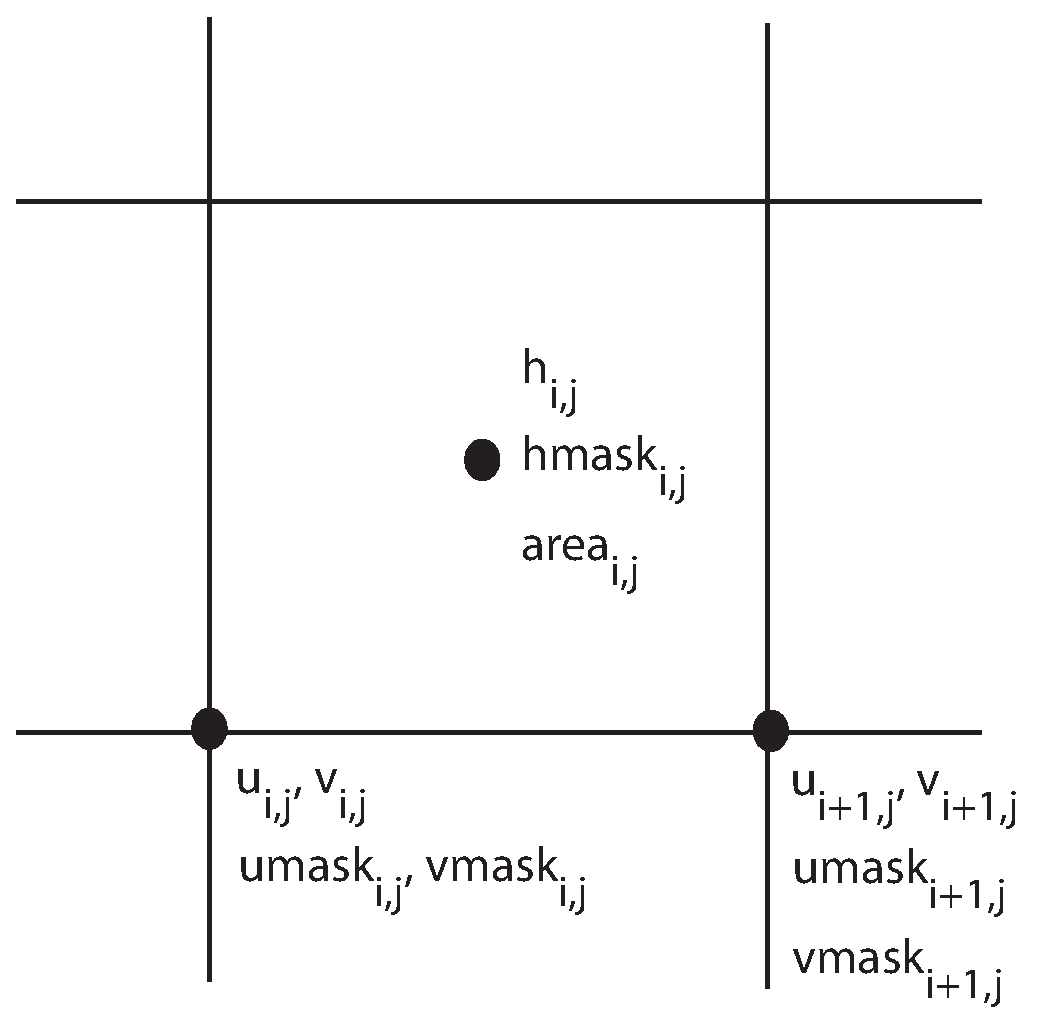
\includegraphics[width=3in]{s_phys_pkgs/figs/stencil.eps}

%\begin{figure}
%\center
%\label{fig:hmask}
%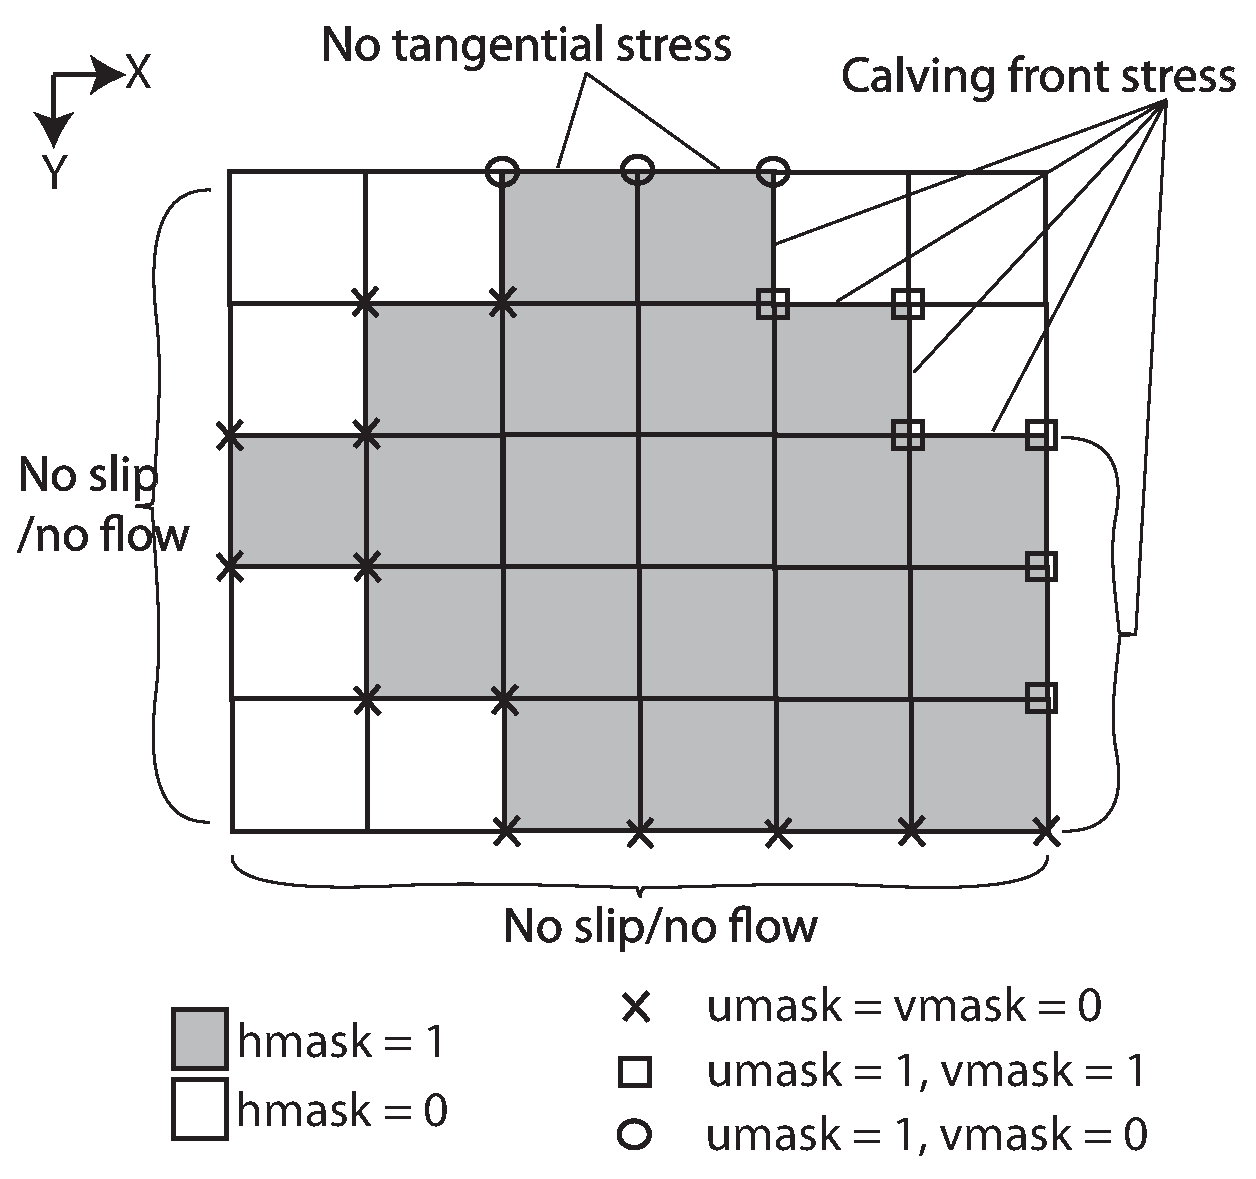
\includegraphics[width=3in]{s_phys_pkgs/figs/mask_cover.eps}
%\end{figure}

\begin{figure}
\begin{center}
\label{fig:stencil}
\resizebox{5.0in}{3.0in}{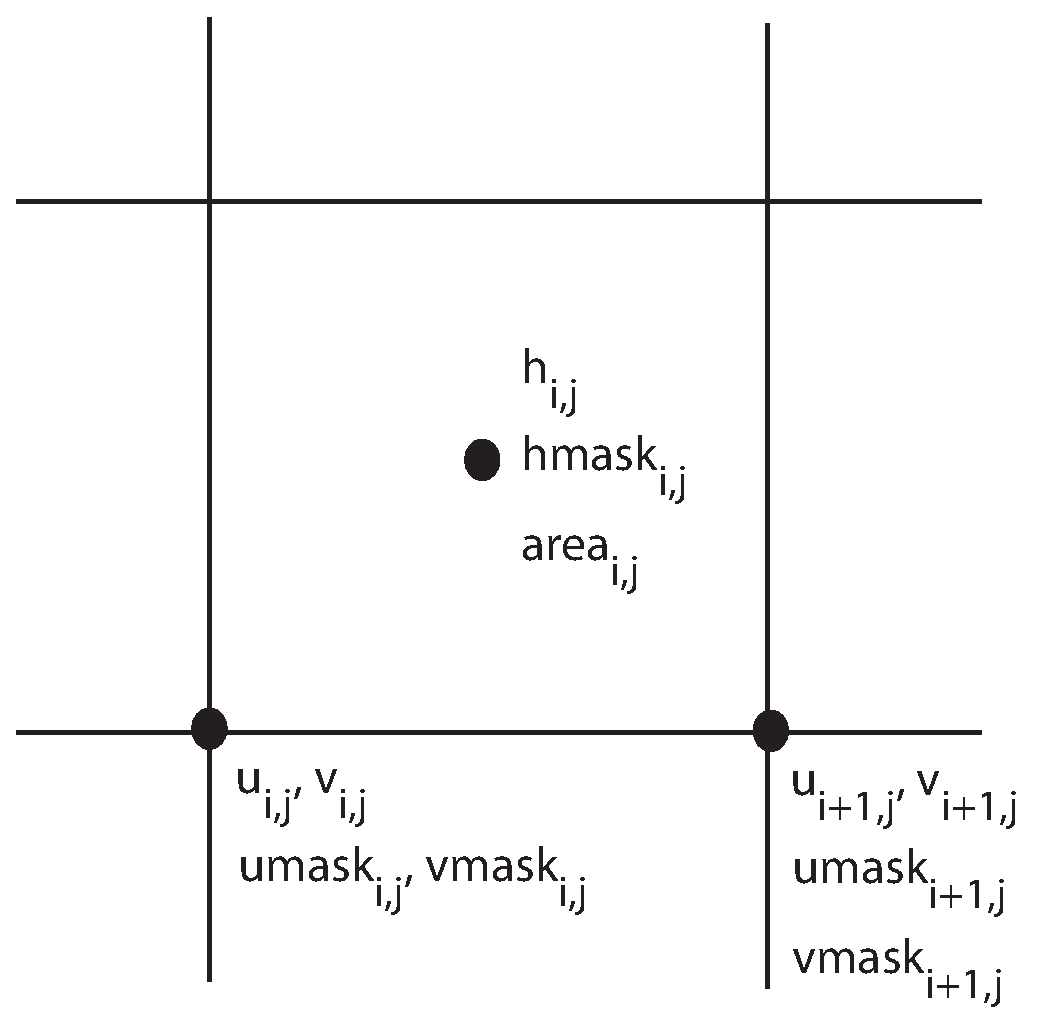
\includegraphics{s_phys_pkgs/figs/stencil.eps}}
\end{center}
\end{figure}

\begin{figure}
\begin{center}
\label{fig:hmask}
\resizebox{5.0in}{3.0in}{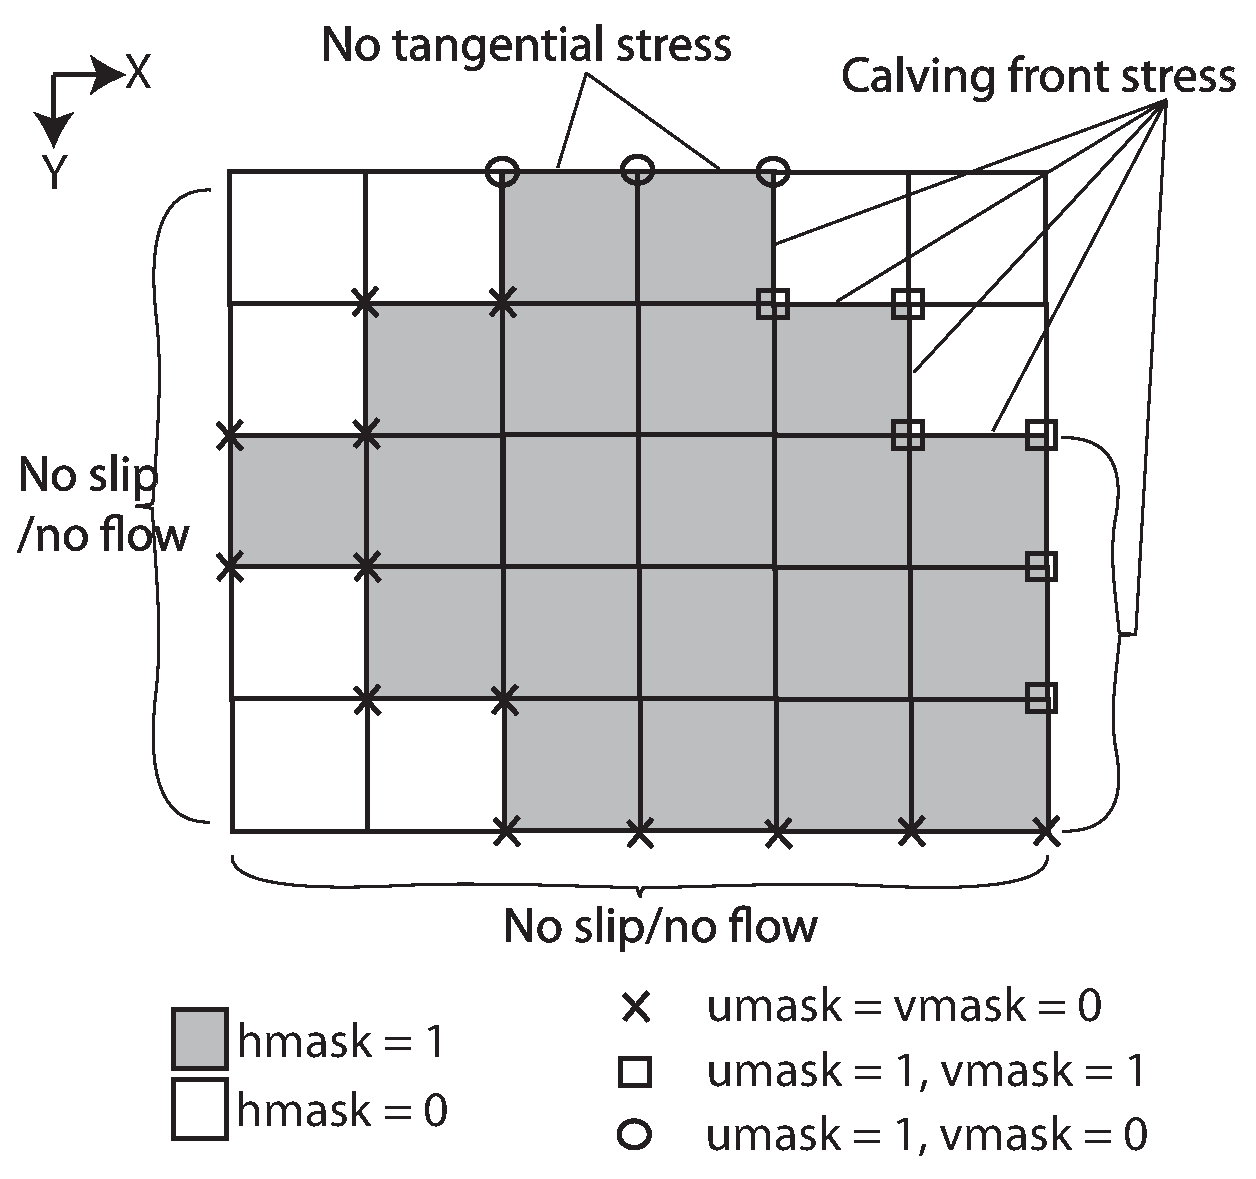
\includegraphics{s_phys_pkgs/figs/mask_cover.eps}}
\end{center}
\end{figure}


\paragraph{Stress/momentum equations}

The stress balance is solved for velocities using a very straightforward,
structured-grid finite element method. Generally a finite element method is used
to deal with irregularly shaped domains, or to deal with complicated
boundary conditions; in this case it is the latter, as explained below. (NOTE:
this is not meant as a finite element tutorial, and various mathematical objects
are defined nonrigorously. It is simply meant as an overview of the numerical
scheme used.)
In this method, the numerical velocities
$u$ and $v$ (or $\overline{u}$, $\overline{v}$ if a hybrid formulation) have a
bilinear shape within each cell. For instance, referring to Fig.
\ref{fig:stencil}, at a point ($x,y$) within cell ($i,j$), and assuming a
rectangular mesh, the $x-$velocity $u$ would be given by 
\begin{align}
 u(x,y) = & (1-\zeta_1)\times(1-\zeta_2)\times u_{i,j}\ + \\
 & (\zeta_1)\times(1-\zeta_2)\times u_{i+1,j}\ + \\
 & (1-\zeta_1)\times(\zeta_2)\times u_{i,j+1}\ + \\
 & (\zeta_1)\times(\zeta_2)\times u_{i+1,j+1},
\end{align}
where
\begin{equation}
 \zeta_1 = x-x_i, \ \  \zeta_2 = y-y_j
\end{equation}
and \textit{e.g.} $u_{i,j+1}$ is the nodal value of $u$ at the top right corner
of the cell. In finite element terms, the functions multiplying a nodal value of
$u$ are the \textit{shape
functions} $\phi$ corresponding to that node, e.g. $\phi_{ij}=\zeta_1\zeta_2$ in cell
($i,j$). Note that $h_{ij}$ is defined at the center of each cell. In the code
velocities are \texttt{U\_STREAMICE} and \texttt{V\_STREAMICE}, and thickness 
is \texttt{H\_STREAMICE}.

If we take a vector-valued function $\Phi=(\phi,\psi)$ which is in the
``solution space'' of ($u,v$) (i.e. $\phi$ and $\psi$ are bilinear in each cell
as 
defined above, and are zero where velocities are imposed), take the dot product
with by (\ref{eq:xmom},\ref{eq:ymom}), and integrate by parts over the domain
$D$, we get the weak form of the momentum equation:
\begin{align}
 -&\int_D \left(h\nu\phi_x (4\dot{\varepsilon}_{xx}+2\dot{\varepsilon}_{yy}) +
h\nu\phi_y \dot{\varepsilon}_{xy} + \beta (u\phi + v\psi) +
h\nu\psi_x\dot{\varepsilon}_{xy} + h\nu\psi_y
(4\dot{\varepsilon}_{yy}+2\dot{\varepsilon}_{xx}) \right) dA = \notag \\
\label{eq:weak1}  & \int_D \Phi\vec{\tau}_d - \int_{\Gamma} \frac{1}{2}g
\left(\rho h^2 - \rho_w R^2\right) \Phi\cdot\vec{n} dS,
\end{align}
where $\Gamma$ is the part of the domain boundary where a calving front stress
condition is imposed, and $\vec{\tau}_d$ is the driving stress 
$\rho g h \nabla s$. Note that the boundary integral does not involve viscosity, or any velocity-dependent terms. This is the advantage of using a finite-element
formulation: viscosity need not be represented at boundaries, and so no complicated one-sided derivative expressions need to be used.

Let $(U,V)$ be the vector of all nodal values
$u_{i,j},v_{i,j}$ that determine $(u,v)$. If we assume that $\nu$ and $\beta$
are independent of $(U,V)$, 
then for any $(\phi,\psi)$, the left hand side of 
\eqref{eq:weak1} is a linear functional of $(U,V)$, i.e. a linear operator that
returns a scalar. We can choose $\phi$ and $\psi$ so that they are nonzero
only at a single node; and we can evaluate \eqref{eq:weak1} for each such
$\phi_{ij}$ and $\psi_{ij}$, giving a linearly independent set of equations for
$U$ and $V$. The left hand side of \eqref{eq:weak1} for each $\phi_{ij}$ and
$\psi_{ij}$ is
evaluated in the subroutine \texttt{STREAMICE\_CG\_ACTION()} in the source file
\texttt{streamice\_cg\_functions.f}.
The right hand side is evaluated in \texttt{STREAMICE\_DRIVING\_STRESS()}. The
latter is not a straightforward
calculation, since the thickness $h$ and the surface $s$ are not expressed by
piecewise bilinear functions, and is discussed below.

\texttt{STREAMICE\_CG\_ACTION()} represents the \textit{action} of a matrix on
the vector represented by $(U,V)$ and \texttt{STREAMICE\_DRIVING\_STRESS()} 
gives the right hand side of a linear system of equations. This information is
enough to solve the linear system, and this is done
with the method of conjugate gradients, implemented (with simple Jacobi
preconditioning) in \texttt{STREAMICE\_CG\_SOLVE()}.

The full nonlinear system is solved in \texttt{STREAMICE\_VEL\_SOLVE()}. This
subroutine evaluates driving stress and then calls a loop
in which a sequence of linear systems is solved. After each linear solve, the
viscosity $\nu$ (the array \texttt{visc\_streamice}) 
and basal traction $\beta$ (\texttt{tau\_beta\_eff\_streamice}) is updated from
the new iterate of $u$ and $v$. The iteration
continues until a desired tolerance is reached or the maximum number of
iterations is reached.

Rather than calling \texttt{STREAMICE\_CG\_ACTION()} each iteration of the conjugate gradient,
the sparse matrix can be constructed explicitly. This is done if \texttt{STREAMICE\_CONSTRUCT\_MATRIX}
is \texttt{\#define}d in \texttt{STREAMICE\_OPTIONS.h}. This speeds up the solution because \texttt{STREAMICE\_CG\_ACTION()}
contains a number of nested loops related to quadrature points and interactions between nodes of a cell.

The driving stress $\tau_d=\rho g \nabla s$ is not as straightforward to deal
with in the weak formulation, as $h$ and $s$ are 
considered constant in a cell. Furthermore, in the ice shelf the driving stress
can be written as
\begin{equation}
 \label{eq:shelf_taud}
 \vec{\tau}_d = \frac{1}{2}\rho g (1-\frac{\rho}{\rho_w})\nabla(h^2).
\end{equation}
Among other things, this (along with equations \ref{eq:cfbcx} and
\ref{eq:cfbcy}) implies that for an unconfined shelf (one for which the only
boundaries are a 
calving front and a grounding line), the stress state along the grounding line
depends
only on the location at depth of the grounding line. The numerical
representation of velocities
must respect this. Thus the driving stress contribution in the $x-$ momentum
equation at node $(i,j)$ is given as follows.
\begin{equation}
 \tau_{d,x}(i,j) = \begin{cases} 
                    \frac{1}{4}\rho g (\gamma_{ij}
h_{ij}+\gamma_{i-1,j}h_{i-1,j})(\gamma_{i-1,j}s_{i-1,j}-\gamma_{ij}s_{ij}) &
\mbox{case I} \\
                    \frac{1}{4} \frac{rA_{i-1,j}}{\Delta x_{f,i-1,j}} g (\rho
h_{i-1,j}^2 - \rho_w b_{i-1,j}^2) & \mbox{case II} \\
                    -\frac{1}{4} \frac{rA_{i,j}}{\Delta x_{f,ij}} g (\rho
h_{ij}^2 - \rho_w b_{ij}^2) & \mbox{case III}.
                   \end{cases}
\end{equation}
where 
\begin{equation}
 \gamma_{ij} = \sqrt{\frac{rA_{ij}}{\Delta x_{f,ij}}},
\end{equation}
$rA_{ij}$ is the area of cell ($i,j$) and $\Delta x_{f,ij}$ is the width of the
cell at its $y-$midpoint. Cases I, II, and III refer to the situations when (I)
both cells ($i,j$) and ($i-1,j$) are in the domain, (II) only cell ($i-1,j$) is
in the domain, and (III) only cell ($i,j$) is in the domain. (The fact that
$\tau_{d,x}(i,j)$ is being calculated means that the implied boundary is a
calving stress boundary, as explained below.) The above expression gives the
contribution
from the cells above node ($i,j$) (in the $y-$direction). A similar expression
gives the contribution from cells ($i-1,j-1$) and ($i,j-1$), and
corresponding expressions approximate driving stress in the $y-$ momentum
equation. In the ice shelf, the case I expressions give approximations for
\eqref{eq:shelf_taud} which are discretely integrable; in grounded ice the
expression need not be integrable, so any errors associated with varying grid
metrics
can be subsumed into the discretization error.

\paragraph{Orthogonal curvilinear coordinates}

If the grid is not rectangular, but given in orthogonal curvilinear coordinates, the evaluation of \eqref{eq:weak1} is not exact, since the gradient of the basis functions are approximated, as we do not have complete knowledge of the coordinate system, only the grid metrics. Still, we consider nodal basis functions that are equal to 1 at a single node, and zero elsewhere in a cell. 

A cell ($i,j$) has separation $\Delta x_{i,j}$ at the bottom and $\Delta x_{i,j+1}$ at the top (referred to as \texttt{dxG(i,j)} and \texttt{dxG(i,j+1)} in the code). So, for instance, for a cell given by $[\xi_1,\xi_2]\times[\eta_1,\eta_2]$, the $\xi$-derivative of the basis function centered at ($\xi_1,\eta_1$) is approximated by
\begin{equation}
\left(\frac{1-q}{\Delta x_{i,j}}\right) + \left(\frac{q}{\Delta x_{i,j+1}}\right)
\end{equation}
where $q$ is the $y$-coordinate of the quadrature point being used. (The code currently uses 2-point gauss quadrature to evaluate the integrals in \eqref{eq:weak1}; with a rectangular grid and cellwise-constant $\beta$ and $\nu$, this is exact.)

Basis function derivatives and quadrature weights are stored in \texttt{Dphi} and \texttt{grid\_jacq\_streamice}. Both are initialized in \texttt{STREAMICE\_INIT\_PHI}, called only once.

\paragraph{Boundary conditions and masks}

The computational domain (which may be smaller than the array/grid as defined by
\texttt{SIZE.h} and \texttt{GRID.h}) is determined by a number of mask arrays 
within the \texttt{STREAMICE} package. They are 
\begin{itemize}
 \item $hmask$ (\texttt{STREAMICE\_hmask}): equal to 1 (ice-covered), 0 (open
ocean), 2 (partly-covered), or -1 (out of domain)
 \item $umask$ (\texttt{STREAMICE\_umask}): equal to 1 (an ``active'' velocity
node), 3 (a Dirichlet node), or 0 (zero velocity)
 \item $vmask$ (\texttt{STREAMICE\_vmask}): similar to umask
 \item $ufacemaskbdry$ (\texttt{STREAMICE\_ufacemaskbdry}): equal to -1
(interior face), 0 (no-slip), 1 (no-stress), 2 (calving stress front), 3
(Dirichlet), or 4 (flux input boundary); when 4, then \texttt{u\_flux\_bdry\_SI} must be initialized, through binary or parameter file
 \item $vfacemaskbdry$ (\texttt{STREAMICE\_vfacemaskbdry}): similar to
ufacemaskbdry
\end{itemize}
$hmask$ is defined at cell centers, like $h$. $umask$ and $vmask$ are defined at
cell nodes, like velocities. $ufacemaskbdry$ and $vfacemaskbdry$ are defined at 
cell faces, like velocities in a $C$-grid - but unless
\texttt{STREAMICE\_GEOM\_FILE\_SETUP} is \texttt{\#define}d in
\texttt{STREAMICE\_OPTIONS.h}, the values are only relevant at the boundaries of
the grid.

Essentially $hmask$ controls the domain; it is specified at initialization and does not change unless calving front advance is allowed.
$ufacemaskbdry$ and $vfacemaskbdry$ are defined at initialization as well. Masks are either initialized through binary files or through the text file \texttt{data.streamice} (see the streamice tutorial)

The values of $umask$ and $vmask$ determine which nodal values of $u$ and $v$ are involved in the solve for velocities. 
Before each call to \texttt{STREAMICE\_VEL\_SOLVE()}, $umask$ and $vmask$ are re-initialized. Values are only relevant if they border a cell where $hmask=1$.
Furthermore, if a cell face is a ``no-slip'' face, both $umask$ and $vmask$ are set to zero at the face's nodal endpoints.
If the face is a Dirichlet boundary, both nodal endpoints are set to 3. If $ufacemaskbdry=1$ on the $x-$boundary of a cell, i.e. it is a no-stress boundary, then 
$vmask$ is set to 1 at both endpoints while $umask$ is set to zero (i.e. no normal flow). If the face is a flux boundary, velocities are set to zero (see ???).
For a calving stress front, $umask$ and $vmask$ are 1: the nodes represent active degrees of freedom.

With $umask$ and $vmask$ appropriately initialized, \texttt{STREAMICE\_VEL\_SOLVE} can proceed rather generally. Contributions to \eqref{eq:weak1} are only
evaluated if $hmask=1$ in a given cell, and a given nodal basis function is only considered if $umask=1$ or $vmask=1$ at that node.

\paragraph{Thickness evolution}

\eqref{eq:contEq} is solved in the subroutine \texttt{STREAMICE\_ADVECT\_THICKNESS}, similarly to the advection routines in MITgcm. Mass fluxes are evaluated, first in the $x$-direction. This is done in the generic subroutine \texttt{STREAMICE\_ADV\_FLUX\_FL\_X}. Flux velocity in the $x-$direction at face ($i,j$) are generated by averaging $u_{i,j}$ and $u_{i,j+1}$. Assuming the flux velocity is positive, if $hmask_{i-2,j},\ mask{i-1,j}$ and $hmask_{i,j}$ are equal to 1, then flux thickness, i.e. the interpolation of $h$ at face ($i,j$), is through a minmod limiter as in the \texttt{generic\_advdiff} package. If these values are not available, then a zero-order upwind flux is used. The exception is when \texttt{STREAMICE\_ufacemask(i,j)} is equal to 4; then \texttt{u\_flux\_bdry\_SI(i,j)} is used for the flux. Fluxes are then differenced to update $h$ in cells that are active ($hmask=1$); a similar procedure follows for the $y-$direction.

\paragraph{Ice front advance}

Flux out of the domain across Dirichlet boundaries is ignored, and flux at no-flow or no-stress boundaries is zero. However, fluxes that cross calving boundaries are stored, and if \texttt{STREAMICE\_move\_front=.true.}, then \texttt{STREAMICE\_ADV\_FRONT} is called after all cells with $hmask=1$ have their thickness updated. In this subroutine, cells with $hmask=0$ or $hmask=2$ with nonzero fluxes entering their boundaries are processed. 

The algorithm is based on \textit{Albrecht} (2011). In this scheme, if cell ($i,j$) fits the criteria, a \textbf{reference} thickness $h_{ref}(i,j)$ is found, defined as an average over the thickness of all neighboring cells with $hmask=1$ that are contributing mass to ($i,j$). The total mass input over the time step to ($i,j$) is calculated as $V_{in}(ij)$. This is added to the volume of ice already in the cell, which is nonzero only if $hmask_{ij}=2$ at the beginning of the time step, and is equal to
\begin{equation}
V_{cell}(i,j) = area_{ij} h_{ij}.
\end{equation}
(If $hmask_{ij}$ is not equal to 1, then $h_{ij}$ has not yet been updated in the current time step.) $area_{ij}$ is stored in the array \texttt{area\_shelf\_streamice}. The total volume, $V_{tot}(i,j)$, is then equal to $V_{cell}(i,j)+V_{in}(i,j)$. Next an effective thickness
\begin{equation}
h_{eff}(i,j) = \frac{V_{ij}}{rA_{ij}}
\end{equation}
is found. If $h_{eff}(ij)<h_{ref}(i,j)$ (but nonzero) then
\begin{itemize}
\item $hmask_{ij}$ is set to 2,
\item $h_{ij}$ is set to $h_{ref}(ij)$,
\item $area_{ij}$ is set to $\frac{V_{tot}(i,j)}{h_{ref}(i,j)}$.
\end{itemize}
If, on the other hand, $h_{eff}(ij)\geq h_{ref}(i,j)$,
\begin{itemize}
\item $hmask_{ij}$ is set to 1,
\item $h_{ij}$ is set to $h_{ref}(ij)$,
\item $area_{ij}$ is set to $rA_{ij}$,
\item Excess flux $q_{ex}(i,j) = V_{tot}(i,j) - h_{eff}(i,j)rA_{ij}$ is found.
\end{itemize}
If $q_{ex}(i,j)$ is zero, nothing more needs to happen. If it is positive, then
\begin{itemize}
\item adjacent cells that are not completely covered ($hmask=0$ or 1) are searched for.
\item if there are no suitable cells, $q_{ex}(i,j)$ is put back into cell ($i,j$) ($h_{ij}$ is set to $h_{ref}(i,j)+\frac{q_{ex}(i,j)}{rA_{ij}}$).
\item if there are suitable cells, $q_{ex}$ is divided \textbf{uniformly} among the corresponding faces of the receiving cells, and the algorithm begins again.
\end{itemize}
The last step is a recursive one; in theory the recursion could continue indefinitely, but in practice at most one recursive call is done. The decision to spread the excess flux uniformly is not the most physically motivated choice, but with appropriate time steps the excess flux value is expected to be small, and is more a matter of mass/volume conservation. This algorithm, while complicated, is necessary for realistic front advance. If newly-covered cells were given full coverage instead of partial coverage and volume were conserved, the front would quickly diffuse.

If \texttt{calve\_to\_mask=.true.}, this sets a limit to how far the front can advance, even if advance is allowed. The front will not advance into cells where the array \texttt{calve\_mask} is not equal to 1. This mask must be set through a binary input file.

No calving parameterisation is implemented in \texttt{STREAMICE}. However, front advancement is a precursor for such a development to be added.

\paragraph{Surface/basal mass balance}

After updating thickness in fully- and partially-covered cells, surface and basal mass balances are applied to nonempty cells. Currently surface mass balance is a uniform value, set through the parameter \texttt{streamice\_adot\_uniform}. Basal melt rates are stored in the array \texttt{BDOT\_streamice}, but are multiplied through by \texttt{float\_frac\_streamice} before being applied.
